\documentclass[12pt]{article}

%% preamble
% ready for submission
\usepackage[preprint]{neurips_2021}
 
% \usepackage[margin=1in]{geometry} 
\usepackage{graphicx}
\usepackage{subcaption}
\usepackage{amsmath,amsthm,amssymb}
\usepackage{color}
\usepackage{fancyhdr}
\usepackage{float}
\usepackage{hyperref}
% \usepackage[round, authoryear]{natbib}
\bibliographystyle{abbrvnat} % aer/natbib/others

\definecolor{dkgreen}{rgb}{0,0.6,0}
\definecolor{gray}{rgb}{0.5,0.5,0.5}
\definecolor{mauve}{rgb}{0.58,0,0.82}

%% environment for coding
\usepackage{listings}
\lstset{frame=tb,
  language=Python,
  aboveskip=3mm,
  belowskip=3mm,
  showstringspaces=false,
  columns=flexible,
  basicstyle={\small\ttfamily},
  numbers=none,
  numberstyle=\tiny\color{gray},
  keywordstyle=\color{blue},
  commentstyle=\color{dkgreen},
  stringstyle=\color{mauve},
  breaklines=true,
  breakatwhitespace=true,
  tabsize=3
}
\newcommand{\code}[1]{\lstinline|#1|}

%% 
%  CUSTOM LATEX MATH COMMANDS 
%% 

%% for vectors, matrices, tensors, and random vectors 
\newcommand{\mVector}[1]
{
    \ifcat\noexpand#1\relax
        \bm{#1}
    \else
        \mathbf{#1}
    \fi
}
\newcommand{\mMatrix}[1]{\mathbf{#1}}
\newcommand{\mTensor}[1]{\bm{\mathscr{#1}}}
\newcommand{\rVector}[1]{\bm{#1}}

%% commands to have blackboard fonts for standard probability stuff (e.g. expected value, variance)
\newcommand{\pr}{\mathbb{P}}
\newcommand{\ev}{\mathbb{E}}
\newcommand{\var}{\mathbb{V}\mathrm{ar}}
\newcommand{\cov}{\mathbb{C}\mathrm{ov}}
\newcommand{\cor}{\mathbb{C}\mathrm{or}}
\newcommand{\bias}{\mathbb{B}\mathrm{ias}}
\newcommand{\R}{\mathbb{R}}
\newcommand{\I}{\mathbb{I}}

%% renewing binomial coefficient, this looks better 
\renewcommand{\binom}[2]{
    \begin{pmatrix}
        #1 \\ #2
    \end{pmatrix}
}

%% command for indicator functions, need bb font for numbers 
\usepackage{bbm}
\newcommand{\ind}{ \mathbbm{1} }

%% defining argmin and argmax functions
\DeclareMathOperator*{\argmax}{argmax}
\DeclareMathOperator*{\argmin}{argmin}

\begin{document}

%% title and authors 
\title{Predicting Future Asset Returns with GCN and LSTM} %replace X with the appropriate number
\author{%
  Wesley Yuan \\
  Department of Statistics \\
  Columbia University \\
  New York, NY, 10027 \\
  \texttt{wy2371@columbia.edu} \\
  \And
  Gurmehar Makker \\
  Department of Statistics \\
  Columbia University \\
  New York, NY, 10027 \\
  \texttt{gm2946@columbia.edu} \\
  \And
  Sierra Vo \\
  Department of Statistics \\
  Columbia University \\
  New York, NY, 10027 \\
  \texttt{tdv2104@columbia.edu} \\
  \And
  Aiden Kenny \\
  Department of Statistics \\
  Columbia University \\
  New York, NY, 10027 \\
  \texttt{apk2152@columbia.edu} \\
}

\maketitle

%% abstract 
\begin{abstract}
Asset price/returns prediction is a widely studied problem in computational finance. Traditional econometrics approaches used time-series models or PDE's to describe single assets behaviors. More recently, deep-learning models that are able to capture temporal relationships, such as Recurrent Neural Networks, have been applied to this problem. However, these typically fail to capture true market dynamics where tradeable assets are linked with others through markets where agents trade multiple assets at once. Therefore, graph models and specifically Graph Neural Networks have been introduced to learn these relationships to produce better results. Several previous studies have shown the promise of this methodology and this work serves to demonstrate the same at a surface level. We adopt the frameworks of previous studies and apply it to a new set of assets and demonstrate the generalizability of the method. We show that the Temporal Graph Convolution (TGC) model outperforms other combination methods and significantly outperforms plain LSTM models. Our code is made available at \href{https://github.com/wesleyyuan17/STAT5242-Project}{https://github.com/wesleyyuan17/STAT5242-Project}
\end{abstract}

%% ----------------------------------------
%  MAIN DOCUMENT 
%% ----------------------------------------

%% introduction 
\section{Introduction} \label{Introduction}

The problem of predicting future returns given historical data for tradable assets has been extensively studied 
with many approaches having been explored. Traditional methods used time-series models such as ARIMA and GARCH to predict future price movements. Similarly, deep-learning models that can take advantage of temporal relations such as Long Short-Term Memory (LSTM) models have been applied to this problem with promising results. 
However, these methods fail to take into account the propagation of information through the market and the correlations of assets. In this aspect, Graph Convolutional Networks (GCN) has demonstrated good performance in regression problems. Combining these should allow for the capture and use of both intra-asset temporal and cross-asset relations to provide superior prediction performance.

\subsection{Related Works} \label{Related Works}

The application of deep learning in asset price predictions is a popular area of ongoing research with most works utilizing variations of Recurrent Neural Network (RNN) models which can learn temporal relationships.

The authors of \cite{Shen2020} develop a custom deep learning pipeline from feature extraction to final prediction. They apply typical transformations such as scaling and calculating technical indicators on price data before combining with company financial data as features that are filtered through recursive feature elimination and PCA before being fed into an LSTM final prediction model. Their work focuses on select single-name stocks from the Chinese stock market and achieves 87\% accuracy on directional predictions on their dataset.

Other works focus on specific parts of the prediction pipeline rather than developing it end-to-end. \cite{Li2018} expand on the vanilla LSTM model to allow for multiple inputs at each step for prediction. The proposed multi-input LSTM model combines low-correlated factors through additional "input gates" (for more detailed description of LSTM model see section \ref{LSTM}). The authors test their architecture on stocks in the CSI-300 index and achieve a 10\% improvement on MSE compared to other state-of-the-art LSTM architectures. Their work shows that additional contextual information can be used to improve performance of stock prediction models.

\cite{Selvin2017} looked to compare the LSTM model with other temporal models such as other RNN architectures as well as sliding window Convolutional Neural Network (CNN) models. The authors tested each of the three models on select single-name stocks (Infosys, TCS, Cipla) and measured their error percentage. They show that deep learning models are able to effectively capture stock price dynamics and that temporal information is highly useful in making future predictions.

The combination of LSTM models and graphical models has been a growing topic of interest as more researchers look to combine the performance of LSTM models in sequential data prediction tasks and the ability of graph models to capture cross-asset dependenceis.

% To do: small write ups on \cite{Matsunaga2019}, \cite{Feng2019}, \cite{Sun2020}, \cite{Hou2021}, and \cite{Peng2021} that combine LSTM and graph models.

\cite{Matsunaga2019} explored the use of temporally-enabled graph models on the stock price prediction problem. In their work, temporal information is added using an LSTM model on raw inputs as an embedding layer that produces inputs for the GCN model. This combination has been named Temporal Graph Convolution (TGC) and aims to produce both sequential and relational embeddings. This embedding and an adjacency matrix calculated using contextual company relationship data are fed into a GCN that outputs some future price prediction. They test their model on the Nikkei 225 and show that it outperforms both the market and, more importantly, the baseline LSTM model by 29.5\% and 6.3\%, respectively.

Similarly, \cite{Feng2019}, makes use of TGC on the related stock ranking problem. That is, rather than predict the raw returns/prices of stocks at some future time horizon, the authors use the TGC model to predict the relative future performance of a set of assets. They test the model on NYSE and NASDAQ stock data and shows it outperforms vanilla GCN and other state-of-the-art ranking algorithms. Their study shows that the superior performance of TGC comes from combining the relational and temporal information and not from either single embedding scheme. Further, their study suggests that TGC's use is not limited to any specific market or regression problem but is trainable on any given set of assets.

\cite{Hou2021} and \cite{Peng2021} further expand on the literature of TGC by testing different methods of constructing the adjacency matrix input. \cite{Hou2021} used a Variational AutoEncoder (VAE) model to cluster stocks into a graph structure and produce some adjacency matrix based on company fundamentals. They tested their adjacency matrix construction method using minute-level data from S\&P100. The authors show superior performance compared to adjacency matrices constructed using raw company fundamentals and using company industry encodings. \cite{Peng2021} also uses industry encodings as an adjacency matrix option but compares it to price-data derived alternatives such as correlation matrix and Dynamic Time Warping (DTW) induced distances. \citeauthor{Peng2021} demonstrated highest performance when using correlation matrix based on 10-day lookback window as the adjacency matrix.

\subsection{Dataset} \label{Dataset}

The dataset used for this project is the G-Research Crypto Dataset which contains minute-level price data for 14 commonly traded crypto assets. For each minute, the open, high, low, and close prices for the past minute are provided as well as the total volume, number of trades, and the volume weighted average price (VWAP). The target variable is the 15 minute return of the given asset. Due to computational constraints, we utilize the latest 100k timestamps available for our study.

In total, about 3\% of the Target values and a near zero number of VWAP values are missing. These missing values are largely the result of insufficient data on assets earlier in the time window from which the data was collected while the last 15 values are all missing (most likely to prevent information leaking). These missing values do not affect our study due to us not utilizing earlier data where the majority of missing values are. The last 15 are forward-filled.

\subsection{Background} \label{Background}

\subsubsection{LSTM} \label{LSTM}

% can cite same papers as Feng2019 if desired

LSTM models are a special kind of Recurrent Neural Network (RNN) model which feature evolving hidden states that capture time-dependencies in sequential inputs. As such, these models have been widely popular in processing sequential data such as speech, text, and video. They solve the main drawback of other RNN models of not being able to caputre long-term dependencies by introducing a "memroy gate" and a "forget gate" to better persist relevant information and discard irrelevant information, respectively. 

A standard LSTM model will have the following components

\begin{enumerate}
	\item Some input at every time step $\mVector{x}_t \in \R^{D_f}$ where $D_f$ is the embedding dimension of the features
	\item A memory state $\mVector{c}_t \in \R^{D_h}$ and a hidden state $\mVector{h}_t \in \R^{D_h}$ where $D_h$ is the number of units in the hidden dimension (typically user-defined)
	\item Input cell $\mVector{i}_t \in \R^{D_h}$ that controls what relevant information from previous states and new input is passed forward
	\item Some intermediate states $\mVector{z}_t, \mVector{c}_t \in \R^{D_h}$
	\item Output cell $\mVector{o}_t \in \R^{D_h}$ that controls what relevant information from intermediate steps makes it to the next time step
	\item Forget cell $\mVector{f}_t \in \R^{D_h}$ that controls what information is discarded going forward
\end{enumerate}

The typical operations in a single LSTM step are as follows

\begin{align*}
\mVector{f}_t & = \sigma(\mVector{W}_f\mVector{x}_t + \mVector{Q}_f\mVector{h}_{t-1} + \mVector{b}_f) \\
\mVector{i}_t & = \sigma(\mVector{W}_i\mVector{x}_t + \mVector{Q}_i\mVector{h}_{t-1} + \mVector{b}_i) \\
\mVector{z}_t & = \tanh(\mVector{W}_c\mVector{x}_t + \mVector{Q}_c\mVector{h}_{t-1} + \mVector{b}_c) \\
\mVector{c}_t & = \mVector{f}_t * \mVector{c}_{t-1} + \mVector{i}_t * \mVector{z}_t \\
\mVector{o}_t & = \sigma(\mVector{W}_o\mVector{x}_t + \mVector{Q}_o\mVector{h}_{t-1} + \mVector{b}_o) \\
\mVector{h}_t & = \mVector{o}_t * \tanh(\mVector{c}_t)
\end{align*}

where $\mVector{W}_* \in \R^{D_h \times D_f}$, $\mVector{Q}_* \in \R^{D_h \times D_h}$, and $\mVector{b}_* \in R^{D_h}$ are learnable parameters and $\sigma$ denotes some user-specified activation function.

\subsubsection{Graph Neural Networks}

% https://distill.pub/2021/gnn-intro/

Graph neural networks (GNN) is the application of neural networks to learning graph problems such as link prediction, node classification, etc. These models have achieved state-of-the-art performance on graph problems as well as regression/classification on data with natural graph structure (such as review data, word nets, social networks, etc.). GNN are typically classified according to the scope of their learning, either node-level or graph-level where graph-level GNN add more sophisticated pooling to node-level GNN to make global predictions. 

GNN's main improvement over standard deep learning methods is the focus on learning embeddings of nodes, edges, or subgraphs that preserve structure such as permutation invariances. This can be done by having separate models for each component of a graph (nodes, edges, global) that are able to better capture information than using a single model on a simpler representations (such as adjacency matrices/lists). A convenient viewpoint is that of the encoder-decoder model taken in \cite{Hamilton2017} where any given task has an encoder that learns the embeddings of the graph components and a decoder that learns the mapping from the embeddings to the targets. Thus, given a graph $\mathcal{G} = (\mathcal{V}, \mathcal{E})$, with $v_i, v_j \in \mathcal{V}$, and $s_{\mathcal{G}}$ being some structure of the graph, the model is given by

\begin{equation}
s_{\mathcal{G}}(v_i, v_j) \approx \text{Decode}(\text{Encode}(v_i), \text{Encode}(v_j))
\end{equation}

For example, setting $s_{\mathcal{G}}(v_i, v_j) = A_{i,j}$ would give the problem of predicting the connections in the graph.

Graph connectivity is utilized in pooling the outputs of these separate models between layers. For node prediction tasks this would entail pooling edge information at the connected node whereas for edge prediction tasks the information is pooled from nodes that the edge connects. This pooling between neighboring components also performs an implicit message passing whereby component embeddings affect the updates of those they are connected to. Let $\mVector{x}_i^{l}$ be the encoding after the $l$-th message passing layer, then the update to the embedding is given by

\begin{equation}
\mVector{x}_i^{l+1} = \mVector{W}^{l}\mVector{x}_i^{l} + \text{Aggregate}(\mVector{x}_j^{l}),\ j \in Ne(v_i)
\end{equation}

where Aggregate is some aggregation function, $\mVector{W}^{l}$ is a learned weights matrix, and $Ne(v_i)$ denotes the neighbors of node $v_i$.

The level of message passing is largely determined by the number of GNN layers, with more layers allowing for greater aggregation) and the aggregation function used in pooling the embeddings (with more complicated aggregation schemes allowing for greater information flow).

GCNs add an additional layer of complexity as it takes in a node feature vector and an adjacency matrix at every step to provide improved context for the message-passing steps. Given the adjacency matrix $A \in \R^{n \times n}$, we add self-connections to get $\mVector{\tilde{A}} = \mVector{A} + \mVector{I}_n$ where $I_n$ is the $n \times n$ identity matrix. We can then construct the diagonal degree matrix $\mVector{\tilde{D}}$ where $\mVector{\tilde{D}}_{ii} = \sum_i\mVector{\tilde{A}}$. Then the propagation rule introduced in \cite{Kipf2017} is

\begin{equation}
f(\mVector{H}^{(l)}, \mVector{A}) = \sigma(\mVector{\tilde{D}}^{-\frac{1}{2}}\mVector{\tilde{A}}\mVector{\tilde{D}}^{-\frac{1}{2}}\mVector{H}^{(l)}\mVector{W}^{(l)})
\end{equation}

where $H^{(l)}$ is the activations of layer $l$ and $H^{(0)} = X$ i.e. the node feature vector and $W^{(l)}$ is a learnable weights matrix.



%% methods 
\section{Methods} \label{Methods}

Traditional asset return predictions utilized time-series models that take into account the temporal nature of trading as sequential decision making. As such, most deep-learning applications in this area have leveraged the temporal aspect of RNN models, particularly LSTM, in making predictions (\cite{Shen2020}, \cite{Li2018}, \cite{Selvin2017}). Therefore, we use a vanilla LSTM model as the baseline model against which we compare our combined methods.

To improve upon the baseline, we introduce a GNN that we use to learn relational information from an implicit graph structure derived from the assets. The connectivity of the assets is evident in the log-returns correlation of the assets in our dataset as seen in figure \ref{fig:asset_corr}. This phenomenon can largely attributed to the fact that agents acting in markets tend to trade many assets at once to get better risk-adjusted returns through diversification. The interactions of these market agents with the assets determines the structure of our market graph representation. This approach is also used in \cite{Matsunaga2019}, \cite{Feng2019}, \cite{Sun2020}, \cite{Hou2021}, and \cite{Peng2021}.

\begin{figure}[H]
	\centering
	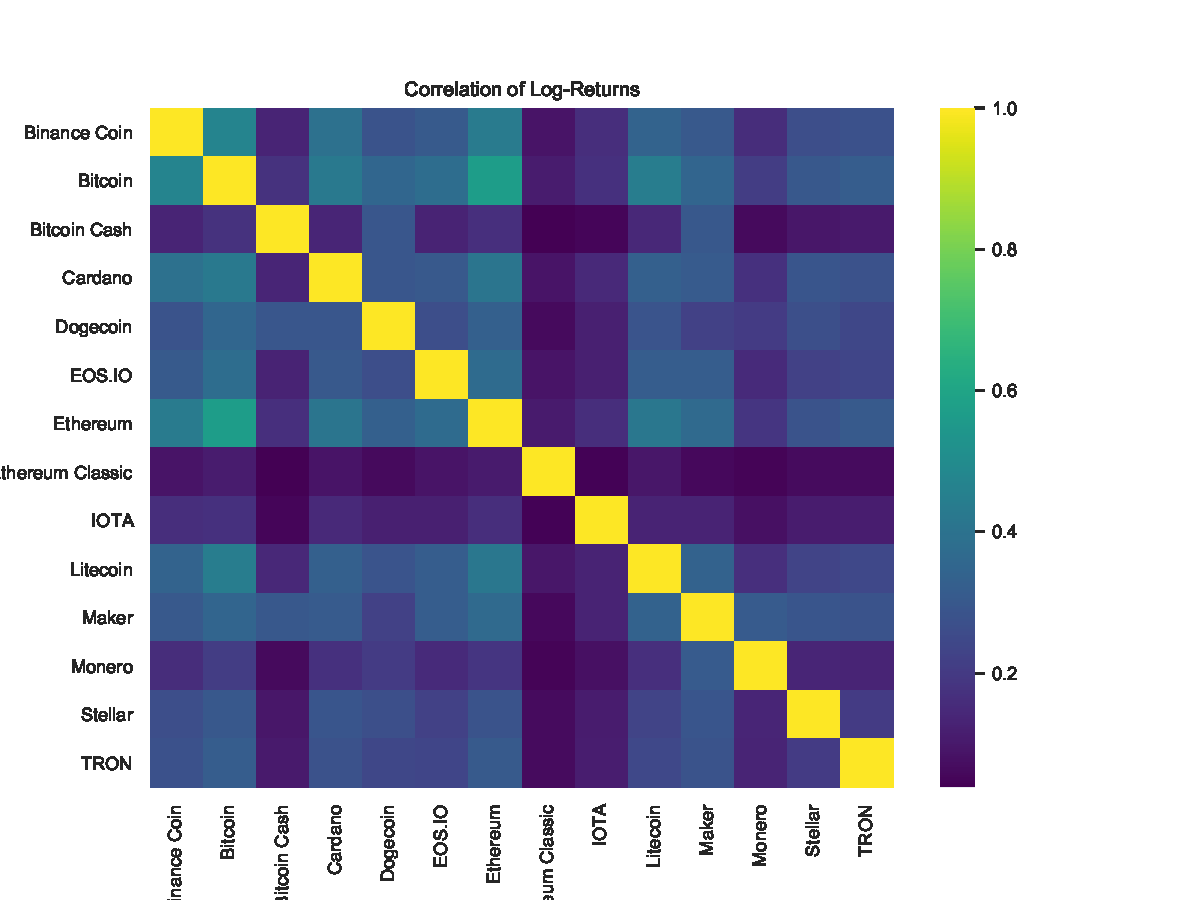
\includegraphics[width=\linewidth]{../../figures/correlation.pdf}
	\caption{Correlation of log returns calculated on minute close prices of assets. Note the high correlation among the most commonly traded assets like Bitcoin/Ethereum and Bitcoin/Binance Coin.}
	\label{fig:asset_corr}
\end{figure}

\cite{Peng2021} show empirically that using the correlation matrix as an adjacency matrix as input into GCN layers provided best performance. Therefore, we use the same, imposing a lookback window equal to the length of the sequence input to the LSTM model. Restricting this lookback window provides a basis for direct comparison as the GCN-augmented model will not have access to more information than the LSTM model and any performance boost would be a result of capturing relational information from the correlation matrix. For our specific GCN model, we implement the propogation rule taken from \cite{Kipf2017} with slight adjustment. For our model, we omit $\tilde{\mVector{D}}^{-1/2}$ from the update rule because it is poorly defined given $\tilde{\mVector{A}}$ as the correlation matrix has negative degree nodes. Therefore, we have the following 

\begin{equation}
f(\mVector{H}^{(l)}, \mVector{A}) = \sigma(\mVector{\tilde{A}}\mVector{H}^{(l)}\mVector{W}^{(l)})
\end{equation}

where variables are as defined above.

%% results 
\section{Experiments}

We use the crypto data described above to train and test the performance of the different models. Due to computational limitations, we take the last 100k time steps with 90k time steps for training and the last 10k used as a test set. Training hyperparameters were tuned manually to find a reasonable best-performing combination.

\subsection{Results}

\begin{figure}[H]
	\centering
	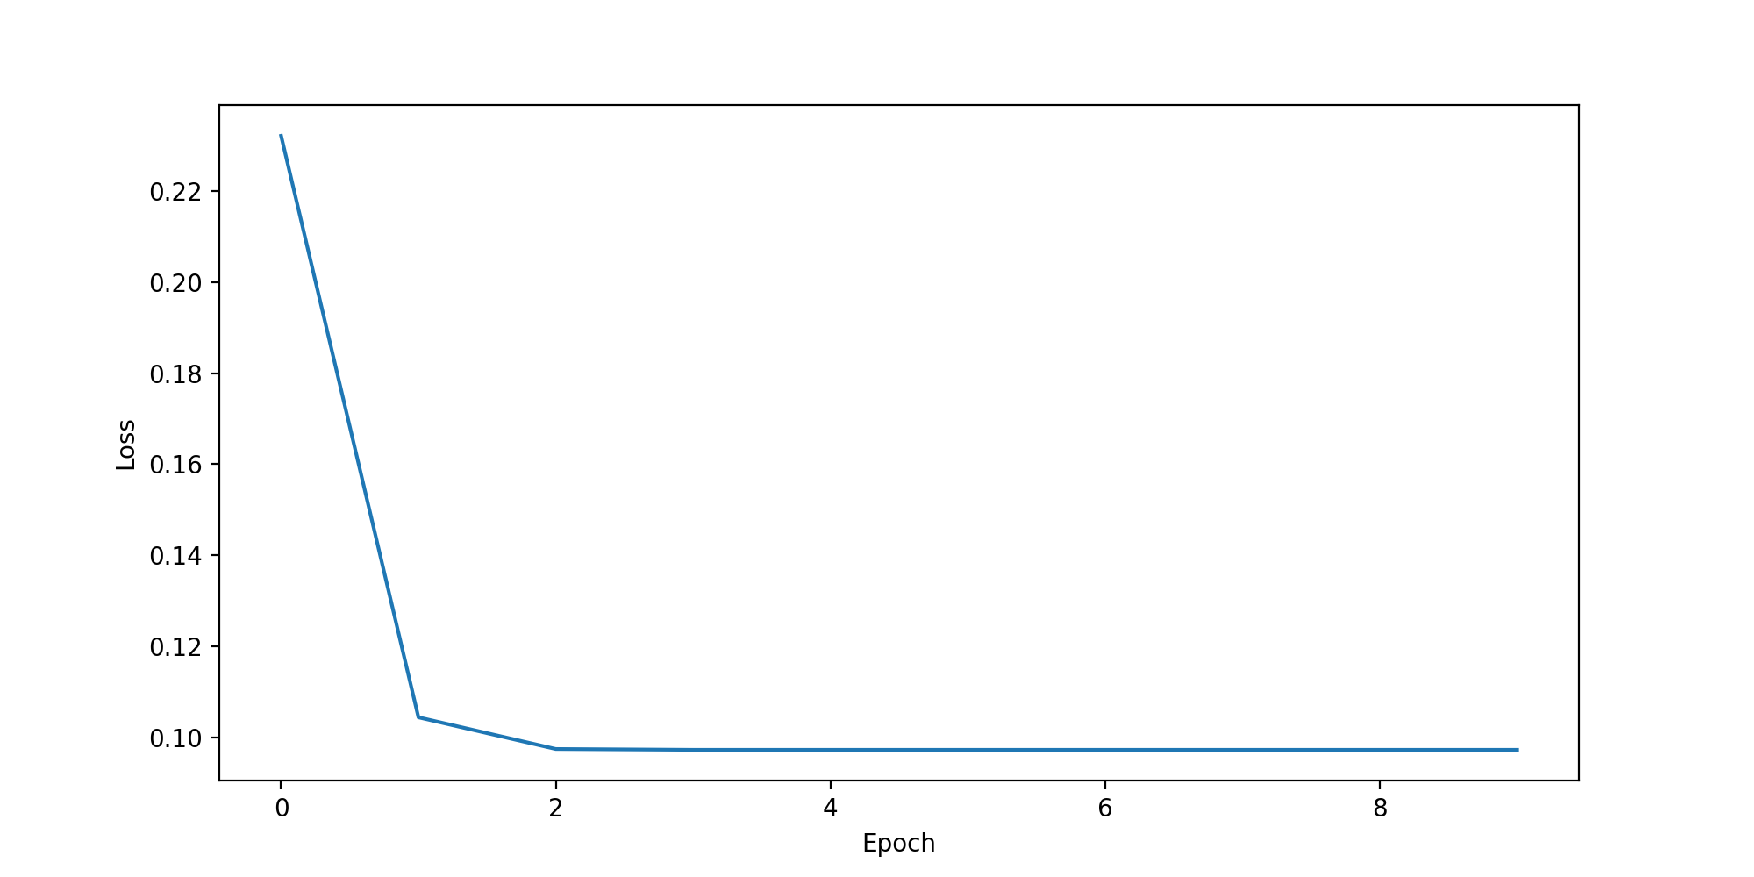
\includegraphics[width=\linewidth]{../../figures/vanilla_lstm_training_loss.pdf}
	\caption{Training loss of baseline LSTM model}
	\label{fig:lstm_loss}
\end{figure}

\begin{table}[H]
	\centering
	\begin{tabular}{|c|c|c|c|c|}
	\hline
	Model & Optimzier & Learning Rate & Momentum & MSE \\
	\hline
	LSTM & SGD & 0.0001 & 0.9 & 0.0030 \\
	Additive & & & & \\
	Sequential & & & & \\
	\hline
	\end{tabular}
	\caption{Hyperparameters for best performing model with average MSE on validation set}
	\label{tab:results_summary}
\end{table}

%% discussion 
\section{Discussion}

Pending results

%% ----------------------------------------
% END OF DOCUMENT 
%% ----------------------------------------

%% bibliography
% \nocite{*}

\bibliography{report}

%% appendix 
\appendix

\section{Appendix}

\end{document}

%% ----------------------------------------
%  NOTES 
%% ----------------------------------------

%  Introduction section: describe the problem you are trying to solve, in 5-7 sentences. It is
% understood that this text may change in the final report, but it doesn’t need to.
% (c) Introduction section: describe the papers that you have read and used to inform your work
% here. Create a bibliography containing these references, and include some sentences on how
% these papers are related and how you used them to build your project. If you used an online
% resource (such as a tf.agents tutorial or something similar) as a starting point, you should
% include that as a reference also.
% (d) Introduction section: describe the data you have for this problem. For example, how many
% training/validation/test samples do you have? What are the dimensionalities of the inputs and
% outputs? If an RL problem, what are the details of the states/actions/rewards?
% (e) Methods section: what is your starting point? For example, will a simple logistic regression
% get you started? What approaches already exist to solve this problem, and how difficult are
% they to implement? Describe in 3-5 sentences what first steps you have taken to start from
% something simple and move to more complex networks. This progression, as we have discussed
% in class on several occasions, is critical to empiricism and working with deep learning.
% (f) Methods section: what architectures/problem setups will you try to get you from this simple
% method to your end goal? For example, will you use dropout or batch normalization, will you
% implement a custom tf.agent, or otherwise? Note it is not necessary to make these choices
% final; this part is about showing progress.
% (g) Results section: what results do you intend to incluude, and why will they demonstrate success?
% Add a list of your intended results and what you hope they will show. If you have early results,
% you may include figures demonstrating the results (optional).
% (h) Discussion section: what are the important takeaways from your work? what problems/opportunity
% for further work (after the semester) do you see for this project? Some of this section will be
% incomplete or speculative since the project is still underway, and that is acceptable (of course
% it should be complete upon final project submission).